\documentclass[12pt,a4paper]{article}

\usepackage[utf8]{inputenc}
\usepackage[T1]{fontenc}
\usepackage{parskip}
\usepackage{amsmath, amssymb, graphicx,pict2e,xcolor}
\usepackage{tcolorbox}
\usepackage{fancyhdr}
\definecolor{bananamania}{rgb}{0.98, 0.91, 0.71}
\pagecolor{bananamania}
\setlength{\headheight}{15.6pt}
\pagestyle{fancyplain}
\graphicspath{{/Users/econhead/NOTES/Probability/ProbClassNotes/13_10_2024/Figures/}}
\fancyhead[L]{Laxman Singh}
\fancyhead[R]{\today}
\usepackage{float}
\floatstyle{boxed}
\restylefloat{figure}

\title{Statistical Inference}

\begin{document}
   \section{Point Estimation}
   
   \subsection{Evaluating Estimators}
   \begin{align*}
    \mathrm{MSE}_{\hat{\Theta}}(\theta)&=\mathbb{E}_{\theta}(\hat{\Theta}-\theta)^2 \\
    &= \mathbb{E}_{\theta}(\hat{\Theta}-\mathbb{E}_{\theta}(\hat{\Theta})+ \mathbb{E}_{\theta}(\hat{\Theta})-\theta)^2\\
    &= \mathbb{E}_{\theta}\left( \hat{\Theta} - \mathbb{E}_{\theta}(\hat{\Theta})\right)^2 + 
    \left( \mathbb{E}_{\theta}(\hat{\Theta}) - \theta \right)^2 \\  
    &= \mathbb{V}_{\theta}(\hat{\Theta})+ (B_{\hat{\Theta}}(\theta))^2
   \end{align*}
    So Mean Squared Error (MSE) is equal to the Variance of the estimator \(\hat{\Theta}\) plus the squared bias of the estimator \(\hat{\Theta}\).

   Suppose \(X_{1},X_{2},\ldots,X_{n} \overset{iid}{\sim} \text{Unif}[0,\theta ]\), where \(\theta>0\) is the unkown parameter. Then find the following; 
   
   \begin{itemize}
    \item \(\hat{\Theta}=\max(X_{1},X_{2},\ldots,X_{n})\).
    \item Check for the unbiasedness and consistency of \(\hat{\Theta}\).
    \item Determine the \(\mathrm{MSE}_{\hat{\Theta}}(\theta)\quad \forall \theta\).     
   \end{itemize}

   We can easily see that the estimator is not unbiased because we are taking the maximum possible value of one particular sample, 
   but \(\max(X_{1},\ldots,X_{n})\leq \theta \) then it's expected value will always fall short of \(\theta\). 
   
   More Precisely, we want to find 
   \begin{equation*}
    \mathbb{E}_{\theta}(\max(X_{1},\ldots,X_{n}))
   \end{equation*}    
   Now,
   \begin{align*}
    F_{\hat{\Theta}}(x)&= Pr_{\theta}(\max(X_{1},\ldots,X_{n})\leq x) \\
    &= (Pr_{\theta}\left( X_{1}\leq x \right))^n \\
    &= \left( \frac{x}{\theta} \right)^n\\
    f_{\hat{\Theta}}(x)&= \frac{nx^{n-1}}{\theta^n},  \quad 0\leq x\leq \theta
   \end{align*}
   So,
   \begin{align*}
       \mathbb{E}_{\theta}\left( \max\left( X_{1},X_{2},\ldots,X_{n} \right)  \right)&= \int_{0}^{\theta} x\cdot \frac{n x^{n-1}}{\theta^n} \mathrm{d}x \\
       &= \left(\frac{n}{n+1}\right)\theta
   \end{align*}    
   Which is clearly less than \(\theta\) and therefore our estimator \( \hat{\Theta}\) is not unbiased.  
   
   Now to check for Consistency we want to show that,
   \begin{equation*}
       \lim_{n\to \infty} \mathbb{P}_{\theta}\left( |\max\left( X_{1},X_{2},\ldots,X_{n} \right) - \theta | > \epsilon \right) =0
   \end{equation*} 
   Now, 
   \begin{align*}
    \mathbb{P}_{\theta}\left( |\max\left( X_{1},X_{2},\ldots,X_{n} \right) - \theta | > \epsilon \right)&= \mathbb{P}_{\theta}\left( \theta - \max\left( X_{1},X_{2},\ldots,X_{n} \right)>\epsilon  \right)\\
    &=\mathbb{P}_{\theta}\left( \max\left( X_{1},X_{2},\ldots,X_{n} \right) < \theta - \epsilon  \right) = \left(\frac{\theta - \epsilon}{\theta}\right)^n
   \end{align*}
   Then,
   \begin{equation*}
    \lim_{n\to \infty}\left(\frac{\theta - \epsilon}{\theta}\right)^n=0 
   \end{equation*}
   and therefore are estimator \(\hat{\Theta}\) is consistent.
   
   
   Now to find the MSE we have to first find the variance of our esstimator, i.e., \(\mathbb{V}_{\theta}(\max\left( X_{1},X_{2},\ldots,X_{n} \right))\) and then \(\left( B_{\hat{\Theta}}(\theta) \right)^2 \);
   
   \begin{align*}
    \mathbb{V}_{\theta}&=\mathbb{E}_{\theta}\left[ \hat{\Theta}^2 \right] - \left( \mathbb{E}_{\theta}\left[ \hat{\Theta} \right]    \right)^2 \\
    &= \int_{0}^{\theta} x^2 \cdot \frac{nx^{n-1}}{\theta^n}\mathrm{d}x
    - \left[\int_{0}^{\theta} x \cdot \frac{nx{n-1}}{\theta^n}\mathrm{d}x\right]^2 \\
    &= \frac{n\theta^2}{(n+1)^2(n+2)}\\
   \end{align*}
   and,
   \begin{align*}
    \left(B_{\hat{\Theta}}(\theta)\right)^2&= (\mathbb{E}_{\theta}[\hat{\Theta}-\theta])^2\\
    &= (\mathbb{E}_{\theta}[\hat{\Theta}]-\mathbb{E}_{\theta}[\theta])^2\\
    &= \frac{\theta^2}{(n+1)^2}
   \end{align*}
   Therefore,
   \begin{align*}
    \mathrm{MSE}_{\hat{\Theta}}(\theta)&= \mathbb{V}_{\theta}(\hat{\Theta})+ \left( B_{\hat{\Theta}}(\theta) \right)^2 \\
    &= \frac{2\theta^2}{(n+1)(n+2)}
   \end{align*}
   
   \begin{figure}[h]
       \centering
       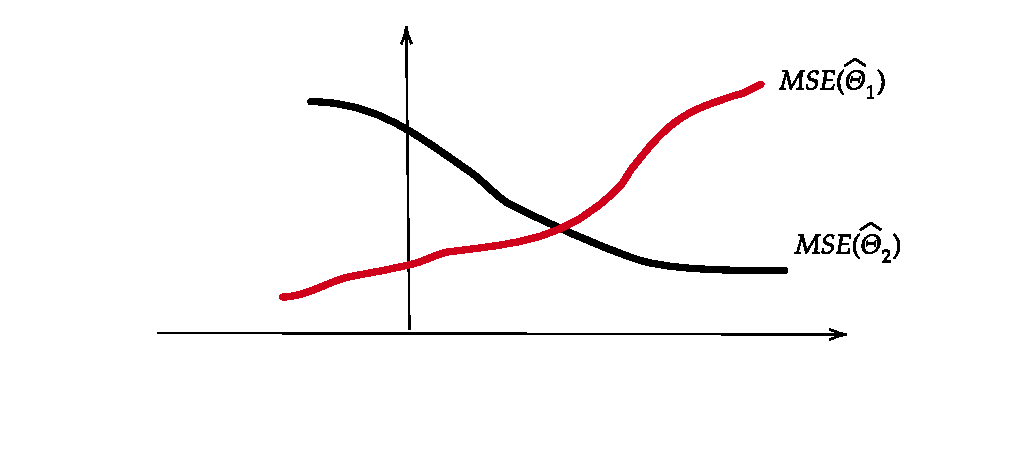
\includegraphics[width=\textwidth]{fig.pdf}
       \caption{Comparing Mean Squared Errors}
       \label{Label}
   \end{figure}
    
   When comparing two estimators such as \(\hat{\Theta}_{1}\) and \(\hat{\Theta}_{2}\), \(\hat{\Theta}_{1}\) is better than \(\hat{\Theta}_{2}\) if;
   \begin{itemize}
    \item \(\mathrm{MSE}_{\hat{\Theta}_{1}}(\theta) \leq \mathrm{MSE}_{\hat{\Theta}_{2}}(\theta) \quad \forall \ \theta\)
    \item \(\mathrm{MSE}_{\hat{\Theta}_{1}}(\theta) < \mathrm{MSE}_{\hat{\Theta}_{2}}(\theta) \quad \text{for some} \ \theta\)    
   \end{itemize}        
    
   
   \paragraph{Question:}
    Suppose \(X_{1},X_{2},\ldots,X_{n} \  \text{are} \ iid \) with \(\mathbb{E}(X_{i})=\mu (< \infty)\) and \(Var(X_{i})=\sigma^2 (<\infty)\),
    Compare the MSE of these estimators for \(\mu\) 

    \begin{itemize}
        \item  \(m_{1}=X_{1}\)
        \item \(m_{2}=\frac{X_{1}+X_{2}}{2}\)
        \item \(m_{n}=\frac{X_{1}+X_{2}+\ldots +X_{n}}{n}\)
    \end{itemize}
    

    Note that all of them have the same expected values, i.e., \(\mathbb{E}(m_{1})=\mathbb{E}(m_{2})=\ldots=\mathbb{E}(m_{n})=\mu\). 
    
    \begin{align*}
        \mathrm{MSE}(m_{1})&=\sigma^2\\
        \mathrm{MSE}(m_{2})&=\frac{\sigma^2}{2}\\
        \mathrm{MSE}(m_{n})&=\frac{\sigma^2}{n}
    \end{align*}
    so the MSE grows smaller as n increases. 
   

    \subsection{Maximum Likelihood Estimator}
    \(X_{1},X_{2},\ldots,X_{n} \ \text{are} \ iid\) random variables from some population \(f(x;\theta )\) where \(\theta\) is the unkown parameter we want to estimate. 
    
    Tak Obseravation \( X_{1},X_{2},\ldots,X_{n}\)  and find the joint density of them which will be the product of the marginals, we call this joint density a Likelihood function,
    \begin{equation*}
        \mathcal{L}(\theta ; x_{1},x_{2},\ldots,x_{n})=f(x_{1};\theta)f(x_{2};\theta) \cdots f(x_{n};\theta)  
    \end{equation*}    
    then we can solve the following;
    \begin{tcolorbox}
    \begin{align*}
         \max_{\theta } & \quad \mathcal{L}(\theta) \\
    \end{align*}
    \end{tcolorbox}
    the solution to the above problem is \(\hat{\Theta}_{MLE}\). 
    
    Now,

    Suppose \(X_{1},X_{2},\ldots,X_{n}\) are \(iid\) Bern\((p)\),then
    estimate \(p\) using MLE;
    \begin{tcolorbox}
    \begin{align*}
        \mathcal{L}(p ; x_{1},\ldots,x_{n})=p^{\sum_{i=1}^{n}x_{i}}(1-p)^{n-\sum_{i=1}^{n}x_{i}}\\
    \end{align*}
    \end{tcolorbox}
    we want to maximise the above but we can take an increasing transformation and solve the following,

     \begin{align*}
           \max_{p}  \quad \ln(\mathcal{L}(p;x_{1},\ldots,x_{n}))&= (\sum_{i=1}^{n}x_{i})(\ln(p))+(n-\sum_{i=1}^{n}x_{i} )(\ln(1-p))\\
           \text{differentiating w.r.t p}; & \quad \frac{\sum_{i=1}^{n} x_{i}}{p} - \frac{n-\sum_{i=1}^{n} x_{i}}{1-p}=0\\
           &\implies \sum_{i=1}^{n} x_{i} - p\sum_{i=1}^{n} x_{i}= np - p\sum_{i=1}^{n} x_{i}\\
           &=\hat{p}_{MLE}=\frac{\sum_{i=1}^{n} x_{i}}{n}
    \end{align*}
     So in this case it turns out to be jsut the sample mean.
    
     \paragraph{Question:}
     Suppose \(X_{1},X_{2},\ldots,X_{n}\overset{iid}{\sim}\mathcal{N}(\mu ,1)\), where \(\mu\) is unknown, find \(\hat{\mu}_{MLE}\).
     
    \begin{align*}
        \mathcal{L}(\mu ; x_{1},x_{2},\ldots,x_{n})&=f(x_{1};\mu)f(x_{2};\mu) \cdots f(x_{n};\mu) \\
        \mathcal{L}(\mu) &= \prod_{i=1}^n f_{X_i}(x_i; \mu) = \left(\frac{1}{\sqrt{2\pi}}\right)^n \exp\left(-\frac{1}{2} \sum_{i=1}^n (x_i - \mu)^2\right)\\
        \ell(\mu) = \log \mathcal{L}(\mu) &= -\frac{n}{2} \log(2\pi) - \frac{1}{2} \sum_{i=1}^n (x_i - \mu)^2\\\frac{d\ell(\mu)}{d\mu} &= \frac{d}{d\mu} \left(-\frac{1}{2} \sum_{i=1}^n (x_i - \mu)^2\right) = \sum_{i=1}^n (x_i - \mu)=0\\
        &\Rightarrow n\mu = \sum_{i=1}^n x_i\\
        &\hat{\mu_{MLE}} = \frac{1}{n} \sum_{i=1}^n X_i        
    \end{align*} 
    This is the sample mean, which makes intuitive sense as the best estimator of the population mean \(\mu\)  .
\end{document}